\documentclass[sigconf]{acmart}
\sloppy
\usepackage{graphicx}
\usepackage{color}
\settopmatter{printacmref=false} % Removes citation information below abstract
\renewcommand\footnotetextcopyrightpermission[1]{} % removes footnote with conference information in first column
\pagestyle{plain} % removes running headers
\makeatletter
\renewcommand\@formatdoi[1]{\ignorespaces}
\makeatother
\settopmatter{printacmref=false}

\usepackage{booktabs} % For formal tables
\setcopyright{none}

\newcommand{\MITAffiliation}{
\affiliation{%
  \institution{Massachussets Institute of Technology}
  \streetaddress{32 Vassar Street}
  \city{Cambridge}
  \state{Massachussets}
  \country{USA}
  \postcode{02139}
}}
 
 \newcommand{\EPFLAffiliation}{
\affiliation{%
  \institution{Swiss Federal Institute of Technology in Lausanne (EPFL)}
  \streetaddress{Route Cantonale}
  \city{Lausanne}
  \country{Switzerland}
  \postcode{02139}
}}

\newcommand{\srm}[1]{\textcolor{red}{{\bf Sam:} #1}}
\newcommand{\ra}[1]{\textcolor{blue}{{\bf ra:} #1}}
\newcommand{\gl}[1]{\textcolor{violet}{{\bf Gl:} #1}}
\begin{document}
\title{ShrinkNets}

\author{Guillaume Leclerc}
\authornote{Visiting Student}
\MITAffiliation
\email{leclerc@mit.edu}

\author{Raul Castro Fernandez}
\MITAffiliation
\email{raulcf@csail.mit.edu}

\author{Samuel Madden}
\MITAffiliation
\email{madden@csail.mit.edu}


% The default list of authors is too long for headers.
\renewcommand{\shortauthors}{G. Leclerc et al.}


%\begin{abstract}
%  Write the abstract at the end !
%\end{abstract}

\maketitle

\section{Introduction}

When designing Neural Networks, finding the appropriate size (width and depth)
is key. In particular, these hyper parameters have a strong correlation with
over/underfitting \srm{give reference} \gl{I did some litterature review and
  actually this statement is quite controversial, should we rephrase ?}. The
main problem is that we have no reliable way to find them [ref]. Decades of
experimentation led to some heuristics [ref] that try to prune that immense
space of possible network sizes.  For example, researchers have used strategies
such as random search \gl{Should we also move the references here if we remove
  the pargraph from the related work ?}, meta-gradient descent and parser trees
to reduce find good parameters without exhaustively exploring the entire
hyper-parameter space. Although these strategies help with finding a good set
of hyper-parameters, they still require a compute-intensive search of the
space.

%However, we are still bound to use costly and sometimes complex methods to
%find reasonable values for these hyper-parameters.

\srm{In this paper, we describe ... -- need to give a high level idea of
  solution, and its benefits.  Would be good to give your system/approach a
  name.}

In this paper we present a method to automatically find an appropriate network
size from a single parameter, drastically reducing the hyper-parameter
dimensionality. The key idea is to \emph{learn} the right network size at the
same time that the network is learning the main task. For example, for an image
classification task, with our approach we can provide the training data to a
network---without sizing it a priori---and expect to end up with a network that
has learnt the task without overfitting \gl{too strong, we do not really have
  any guarantee on the generalization, how about changing it to: to end up with
  a network that learnt a tradeoff between size and accuracy}. This approach
has two main benefits. First, we do no longer need to choose a network size
before training.  Second, the final network size will be appropriate for the
task at hand, and not larger \gl{Should we talk about the fact that it automatically gets rid of dead neurons ?}. This is important because oversized networks have
a lower inference throughput and higher  memory footprint.

Our approach has two main challenges. First, on how to dynamically size the
network during training. Second, on how to find a loss function that optimizes
for the additional task of sizing, without deteriorating the learning
performance of the main task. We describe next ShrinkNets, which cope with both
challenges:

% \subsection{Main Contributions}
% 
% The main contribution of this article are:
% \begin{itemize}
%   \item The Filter layer, a neural network layer which puropose is to allow feature selection
%   \item To the best of our knowledge, the first attempts to dynamically change the number of channels in deep convolutional neural networks
%   \item A deep learning library built on top of PyTorch that allow partictionners to train shrinking networks (Feed-Forward and Convolutional)
% \end{itemize}
% 

\section{ShrinkNets}

\srm{Describe our key approach at a high level -- i.e., add a new layer to the
network, called the {\it filter layer}, which ... }

Our approach consists of starting the training process for the task of interest
with an explicitly oversized network. Then, as training progresses, we learn
which neurons are not contributing to learning the main task and remove them
dynamically, thus shrinking the network size. This method requires two building
blocks. First, a way of identifying neurons that are not contributing to the
learning process, and second a way of balancing the network size and the
generalization capability for the main task. We introduce a new layer, called
\textsf{Filter}, which takes care of \emph{deactivating} neurons. We also modify
existing loss functions to incorporate a new term that takes care of balancing
network sizing and generalization capability appropriately. We explain them
next:

%\subsection{Motivation}
%
%\srm{This makes what we have done sound like an incremental change over prior
%work.  Instead, move this description to prior work and say why its not a good
%approach there, then describe what we do as a new method.  }
%
%The method described in [ref] grows and shrinks the network over time. Though
%this seems to be an attractive property to have, during our experiments and
%according to their results, models are very slow to train and sometimes
%converge to suboptimal solutions. Their method also requires a new optimizer
%\textit{AdaRad}.  Our goal was to provide a solution that can easily be
%integrated in existing machine learning systems and provide similar convergence
%speed and accuracy. Therefore, designing a new layer that only allow shrinking
%seemed to be best approach.
%

%\subsection{Definition}

\textbf{Filter Layer: } 

Filter layers have weights in the range $[0,+\infty]$ and are placed after
linear and convolutional layers of traditional deep networks \gl{This is how I
  used it but with the new implementation we can be more creative and put them
  anywhere, should we say "usually placed" insdead ?}. The \textit{Filter
  Layer} takes an input of size $\left(B \times C \times D_1 \times \dots
  \times D_n\right)$, where $B$ is the batch size, $C$ the number of features
(or channels), and $D$ any additional dimension. This structure makes it
compatible with fully connected layers with $n=0$ or convolutional layers with
$n=2$. Their crucial property is a parameter $\theta \in \mathbb{R}^C$, defined
as follows: \srm{Need to define B, C, D} \gl{=> done}.  

\begin{equation} Filter(I;\theta) = I \circ \max(0, \theta) \end{equation}

Where $\circ$ is the Hadamard product (pointwise multiplication) \gl{Should we
  keep only one of them to be more concise ?}, and $\theta$ is expanded in all
dimensions except the second one to match the input size. It is easy to see
that if for any $k$, if $\theta_k \leq 0$, the $k^{\text{th}}$ feature/channel
will forever be $0$. When this happens, we say the Filter layer disables the
neuron. These disabled neurons/channels can be removed from the network without
changing its output (we describe how we perform this removal below). We explain
next how the weights of the Filter Layer are adjusted during training.

%We can use this property to devise a training procedure.

\srm{Give an English description of what this formalism
achieves -- what does the filter layer do, why is it significant.}

%To train networks we need start with a substantially oversized network, then we
%insert \textit{Filter Layers}  (usually after every linear or convolutional
%layer except the last one) and we sample their weight from the
%$\text{Uniform}(0, 1)$ distribution. 

%The \textit{Filter Layer} takes an input of size $\left(B \times C \times D_1
%\times \dots \times D_n\right)$ so it is compatible with fully connected layers
%with $n=0$ or convolutional layers with $n=2$. This layer has a parameter
%$\theta \in \mathbb{R}^C$ and is defined the following way. \srm{Need to define
%B, C, D}.  
%
%\begin{equation} 
%Filter(I;\theta) = I \circ \max(0, \theta)
%\end{equation}
%
%Where $\circ$ is the Hadamard product (pointwise multiplication), and $\theta$
%is expanded in all dimensions except the second one to match the input size. It
%is easy to see that if for any $k$, if $\theta_k \leq 0$, the $k^{\text{th}}$
%feature/channel will forever be $0$. We can use this property to devise a
%training procedure.  
%
%\srm{Give an English description of what this formalism
%achieves -- what does the filter layer do, why is it significant.}

%\subsection{The training procedure}
\textbf{Training Procedure: } Once Filter layers are placed in a deep network, 
%To train networks we need start with a substantially oversized network, then we
%insert \textit{Filter Layers}  (usually after every linear or convolutional
%layer except the last one) and we sample their weight from the
%$\text{Uniform}(0, 1)$ distribution. 
we could train it directly and it
would be equivalent to a normal neural network. However, our goal is to find the
smallest network with reasonable performance. We achieve that by introducing
sparsity in the parameters of the \textit{Filter Layers}. Indeed, having a negative component in the $\theta$ parameter of the filter layer permamently disable its associated feature \gl{Maybe redundant ? we talked about that in the previous paragraph}
. To obtain this sparsity, we simply redefine the loss function:

\begin{equation}
  L'(x,y;\theta) = L(x, y) + \lambda|\theta|
\end{equation}

This choice come from the Lasso loss [ref] and we use it for the same reason:
it introduces sparsity. The bigger the $\lambda$ the more entries in $\theta$
are set to zer, and since zeros entries in $\theta$ correspond to dead neurons,
lambda effectively control the number of neurons/channels in the entire
network. \srm{Again give some intuitive description of what is novel /
  important about this choice of loss function and learning process.  It's hard 
  to understand what is interesting/important about what you have done without
  you explicitly calling it out.} \gl{Is it better this way ?}

Next, we explain how to implement ShrinkNets efficiently.

\section{Software architecture}

\ra{this can be shorter. I'd add it as a third paragraph above, immediately
above the eval}

\gl{Here is a shorter (clearer ?) version:}

\par \textit{Filter Vectors} can easily be implemented in a few lines of code
in many existing deep learning frameworks. However, in ShrinkNets we assume
that we start with obviously oversized networks. If disabled neurons are not
quickly removed, the overhead might caused the training process to be
significantly slower than classic neural networks. This is why we want to
support what we call garbage collection: removing the weights in the layers
that are responsible(or using) features that are disabled.
\par To be able to catpure this relationship between layers we agumented
\textit{Pytorch} (the framework we used as the foundation of our implementation)
with a graph structure very similar to the one available in Keras [ref].
In this graph edges are effectively event hubs responsible for propagating
\textit{feature removal} events to subscribing layers. ShrinkNet layers are
agumented to emit and react to these events but also propagate the event
further if has an impact at the other endpoint of the layer (input or output).
\par This event-based implementation coordinated by edges makes it very easy
to integrate new layers in the library. We even provide automatic wrapping
for layers from pytorch if they have no internal state. For more complex ones,
we provide utilitaries that makes the implementation very concise.


\section{Evaluation}
\subsection{Convergence}

To demonstrate that the approach is viable, we will first show that Shrinking
Networks converge. For this experiment we trained a one hidden layer neural
network with one filter layer to control the number of hidden units. We
initialized the models with $10000$ neurons and trained them on \texttt{MNIST}
using different regularization factors ($\lambda$). We summarized the results in
\autoref{convergence_plot}. [Should we explain the results ?] \srm{Yes, you need
to explain in detail -- what does this show?  How does it prove that your
approach works / is a good idea?}

\begin{figure}
\begin{center}
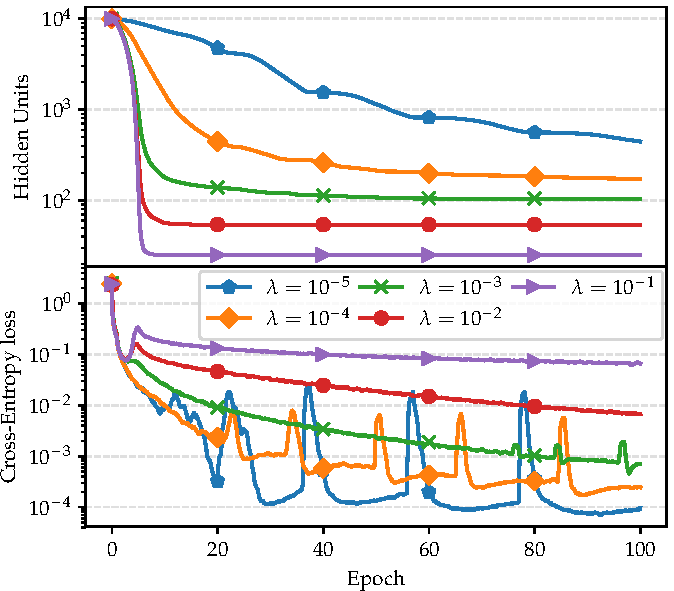
\includegraphics[width=0.5\textwidth]{convergence}
\caption{Evolution of the number of hidden units and loss over time on the \texttt{MNIST} dataset for different $\lambda$ values \label{convergence_plot}}
\end{center}
\end{figure}

\begin{figure}
\begin{center}
  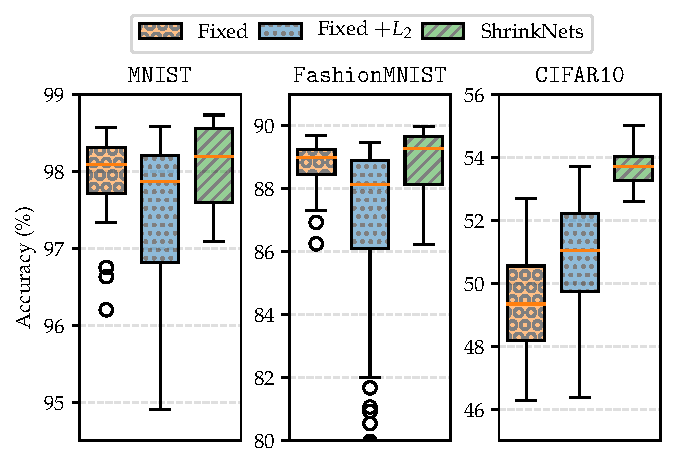
\includegraphics[width=0.5\textwidth]{hyper_opt}
\caption{Distributions of the testing accuracy for different training methods, datasets and architectures using random search\label{hyper_opt_res}}
\end{center}
\end{figure}

\subsection{Comparison between Shrinking and classic Networks}

To demonstrate the value of ShrinkNets in the context of hyper-parameter
optimization we set up the following experiment: We consider two different
architectures, a three hidden layer feed forward network and a \textit{LeNet-5}
[ref]. We do not know the number of channels and neurons and we want to find the
best architecture by performing random search on the parameters that define the
size. For classic neural networks these parameters are the number of channels
and/or neurons; for ShrinkNets there is only one parameter, $\lambda$. We
sampled 50 models of each and trained them, picked the best epoch according to
the validation accuracy and measured their performance on the testing set. Since
ShrinkNets can be considered to be regularized in some sense, to make the
comparison fair we also considered static networks with an $L2$ regularization
factor (also drawn randomly) \srm{L2 regularization over what?}. We summarized
the accuracy we obtained on \autoref{hyper_opt_res}. [Should we explain the
results] \srm{Yes, need to describe in detail -- how does this prove that your
method works/ is a good idea?  What are the key takeaways?}

\section{Related Work}

\ra{I'd remove this paragraph because we used it in the motivation already}
\par In the literature we can see different ways of approaching this issue. The
first one is to select parameters, train the model, evaluate it, repeat and pick
the best one. There are many different ways of selecting parameters: random
search [ref], grid search [ref], meta gradient descent [ref], Parsen trees[ref],
Gaussian processes [ref] etc... but they all suffer from one major drawback: we
have to train and evaluate a very large number of models; and even if some
algorithms allow parallel evaluations [ref] to reduce the overall training time,
the hardware and energy cost is still very significant.  

\ra{I'd argue these techniques are aimed to improve inference time and not to
avoid hyper-parameter optimization}
\par To reduce the number of models trained, another approach is to train a
slightly bigger model and after convergence, remove as many parameters as
possible without impacting the performance of the model. Notable contributions
are Optimal Brain Damage [ref], Deep Compression [ref], and Group sparsity [ref]
(this one is especially related to this article). These techniques are very
interesting but they still require a reasonable network size to start with, so
they usually have to be combined with classic hyper-optimization techniques.  

\srm{How is this shrinking
approach different than previous approaches like Optimal Brain Damage, Deep
Compression,e tc?} 

\par However, some recent contributions like Non-Parametric Neural Netowrks
[ref] and [ref] try to learn the network size (width for the former and depth
for the latter) during the training process and without any prior assumption
about the network size. \ra{revise next}This method dynamically grows and shrinks the network
over time. Though this seems to be an attractive property to have, during our
experiments and according to their results, models are very slow to train and
sometimes converge to suboptimal solutions. Their method also requires a new
optimizer \textit{AdaRad}. \ra{explain how difficult is to get the optimizer
stable. that's a drawback of the method} \ra{Instead, ShrinkNets work out of the
box with existing libraries and does not need any changes to the optimizer.}

\srm{Give a short sentence about how our approach is
different than these previous approaches.} 

\section{Future work}

\ra{this can be shorted, and used as conclusions}

\par Even though the firsts results this technique yields seem promising, there
are many area that we could explore to improve it. In the current implementation
we only "learn" the number of features (neurons or channels). We could try to
augment it with dynamic number of layers as seen in [ref] to be able to
determine the entire architecture.  \par We saw on Figure \ref{convergence_plot}
that the loss temporarily suffers from the removal of neurons. It is likely that
the loss would be more stable if the number of neurons converged faster or
neurons disappeared slower. For this reason we plan to explore proximal gradient
methods to optimize the filter vectors and/or randomize neuron removals.  \par
During our evaluation we picked small datasets mainly to be able to train many
models and have statistically significant distributions. With more computation
resources and time, we could see if it generalizes to bigger datasets and other
architectures like \texttt{ResNet} [ref] (small modifications to the existing
code base are required to support them)

\section{Conclusion}
Do the conclusion at the end

\bibliographystyle{ACM-Reference-Format}
\bibliography{sample-bibliography}

\end{document}
